%
% 44-hauptwert.tex -- Hauptwert
%
% (c) 2026 Prof Dr Andreas Müller
%
\subsection{Hauptwert
\label{buch:integration:residuen:subsection:hauptwert}}
Die Berechnung des Integrals in
Abschnitt~\ref{buch:integration:residuen:section:beispiel}
hat einen Weg verwendet, der den Nullpunkt in einem grossen
Bogen umrundet hat.
So wurde das Integral zwischen $-R$ und $R$ zu einem Wegintegral
über eine geschlossene Kurve vervollständigt, wodurch sich der
Integralsatz anwenden liess.
Auf diese Weise konnte ein uneigentliches Integral von 
$1/(x^2+1)$ über die ganze reelle Achse berechnet werden.

Auch das Integral
%
% fig-sinxx.tex
%
% (c) 2026 Prof Dr Andreas Müller
%
\begin{figure}
\centering
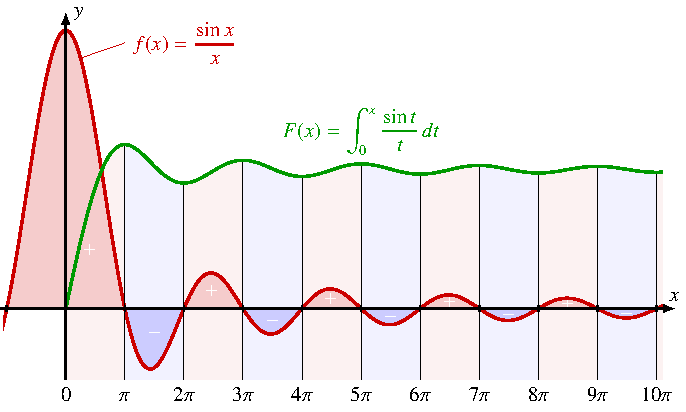
\includegraphics{chapters/030-integration/images/sinxx.pdf}
\caption{Die Stammfunktion von $f(x) = \sin(x)/x$ oszilliert, die Extrema
befinden sich bei den Nullstellen des Integranden, die ganzzahlige
Vielfache von $\pi$ sind.
\label{buch:integration:fig:sinxx}}
\end{figure}
%
\begin{equation}
I
=
\int_{-\infty}^\infty \frac{\sin x}{x}\,dx
\label{buch:integration:residuen:eqn:sinxxintegral}
\end{equation}
ist uneigentlich.
Da der Integrand mit Nullstellen bei ganzzahligen Vielfachen
von $\pi$ oszilliert, nimmt die Stammfunktion
\[
x
\mapsto
F(x)
=
\int_{0}^{x} \frac{\sin t}{t}\,dt
\]
lokale Extrema bei diesen Nullstellen an
(Abbildung~\ref{buch:integration:fig:sinxx}).
Jeder Wert liegt daher zwischen Werten
\[
F\biggl(
\biggl\lfloor\frac{x}{\pi}\biggr\rfloor\pi
\biggr)
=
\int_{0}^{\lfloor\frac{x}{\pi}\rfloor\pi}
\frac{\sin t}{t}\,dt
\qquad
\text{und}
\qquad
F\biggl(
\biggl(\biggl\lfloor\frac{x}{\pi}\biggr\rfloor+1\biggr)\pi
\biggr)
=
\int_{0}^{\left(\lfloor\frac{x}{\pi}\rfloor+1\right)\pi}
\frac{\sin t}{t}\,dt
\]
der Stammfunktion an den nächstliegenden ganzzahligen Vielfachen von $\pi$.
Die Konvergenz des uneigentlichen Integrals ist damit gesichert.
Trotzdem bleibt die Berechnung des Integralwertes offen, da es
keine geschlossene Form für die Stammfunktion gibt.

Um den Werte des Integrals $I$ mithilfe eines Wegintegrals zu berechnen,
muss ein komplexer Integrand und ein passender Weg gefunden werden.
Dabei ist zu berücksichtigen, dass der Integrand an der Stelle $x=0$
eine Singularität hat.
%
% fig-hauptwert.tex
%
% (c) 2026 Prof Dr Andreas Müller
%
\begin{figure}
\centering
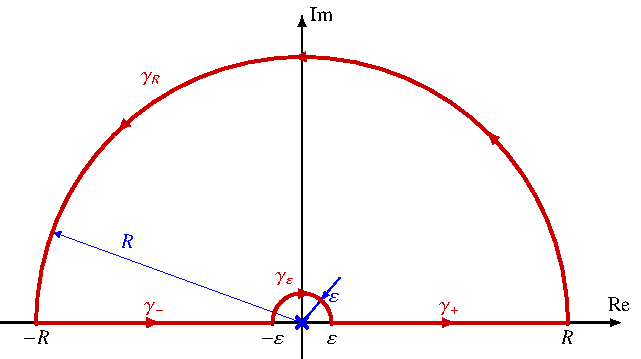
\includegraphics{chapters/030-integration/images/hauptwert.pdf}
\caption{Weg zur Berechnung des Integrals
\eqref{buch:integration:residuen:eqn:sinxxintegral}
mit Hilfe des Weges $\gamma$, der sich aus einem grossen
Kreis mit Radius $R$ und einem kleinen Kreis mit Radius
$\varepsilon$ zusammensetzt.
Dadurch wird die Singularität des Integranden $e^{iz}/z$ an der Stelle
$z=0$ gemieden.
\label{buch:integration:residuen:fig:hauptwert}}
\end{figure}
%
Als Integrand bietet sich
\[
f(z)
=
\frac{e^{iz}}{z}
\]
an.
Während der ursprüngliche reelle Integrand an der Stelle $x=0$ stetig
ist, hat $f(z)$ dort einen Pol.
Als Weg kann der in
Abbildung~\ref{buch:integration:residuen:fig:hauptwert}
dargestellte Weg verwendet werden.
Er setzt sich zusammen aus den beiden Segmenten $[\varepsilon,R]$
und $[-R,-\varepsilon]$ und den Kreisbögen $\gamma_R$ und
$\gamma_\varepsilon$ mit Radien $R$ und $\varepsilon$,
die die Segmente zu einem geschlossenen Weg verbinden.
Im Inneren dieses Weges ist $f(z)$ eine holomorphe Funktion.
Nach dem Integralstatz verschwindet das komplexe Wegintegral
\begin{equation}
\int_{\gamma_+\cdot\gamma_R\cdot\gamma_-\cdot\gamma_\varepsilon} f(z)\,dz
=
\int_{\gamma_+} f(z)\,dz
+
\int_{\gamma_R} f(z)\,dz
+
\int_{\gamma_-} f(z)\,dz
+
\int_{\gamma_\varepsilon} f(z)\,dz
=
0
\label{buch:integration:residuen:eqn:summe}
\end{equation}
über den ganzen Weg.
Das gesuchte Integral $I$ ist der Teil über die beiden Segmente
$\gamma_\pm$ im Grenzwert
\begin{align*}
I
&=
\lim_{R\to\infty}
\lim_{\varepsilon\to 0}
\biggl(
\int_{\gamma_+}
f(z)\,dz
+
\int_{\gamma_-}
f(z)\,dz
\biggr)
\intertext{für $R\to\infty$ und $\varepsilon\to 0$.
Aus \eqref{buch:integration:residuen:eqn:summe} kann man dann
schliessen, dass das Integral auch}
&=
-
\lim_{R\to\infty}
\int_{\gamma_R} f(z)\,dz
-
\lim_{\varepsilon\to 0}
\int_{\gamma_{\varepsilon}} f(z)\,dz
\end{align*}
ist.
Diese Vorgehensweise berechnet das Integral entlang der
reellen Achse mit symmetrischen Segmenten, während
die Definition eines uneigentlichen Integrals verlangt, dass für
die beden Grenzen unabhängig voneinander ein Grenzübergang durchgeführt
wird.
Der symmetrische Grenzwert heisst auch der \emph{Hauptwert} des
Integrals und wird im Kapitel~\ref{chapter:hauptwert} ausführlicher 
dargestellt.




